\documentclass[]{article}
\usepackage{lmodern}
\usepackage{amssymb,amsmath}
\usepackage{ifxetex,ifluatex}
\usepackage{fixltx2e} % provides \textsubscript
\ifnum 0\ifxetex 1\fi\ifluatex 1\fi=0 % if pdftex
  \usepackage[T1]{fontenc}
  \usepackage[utf8]{inputenc}
\else % if luatex or xelatex
  \ifxetex
    \usepackage{mathspec}
  \else
    \usepackage{fontspec}
  \fi
  \defaultfontfeatures{Ligatures=TeX,Scale=MatchLowercase}
\fi
% use upquote if available, for straight quotes in verbatim environments
\IfFileExists{upquote.sty}{\usepackage{upquote}}{}
% use microtype if available
\IfFileExists{microtype.sty}{%
\usepackage{microtype}
\UseMicrotypeSet[protrusion]{basicmath} % disable protrusion for tt fonts
}{}
\usepackage[margin=1in]{geometry}
\usepackage{hyperref}
\hypersetup{unicode=true,
            pdftitle={Simulation},
            pdfauthor={Liu Huihang},
            pdfborder={0 0 0},
            breaklinks=true}
\urlstyle{same}  % don't use monospace font for urls
\usepackage{color}
\usepackage{fancyvrb}
\newcommand{\VerbBar}{|}
\newcommand{\VERB}{\Verb[commandchars=\\\{\}]}
\DefineVerbatimEnvironment{Highlighting}{Verbatim}{commandchars=\\\{\}}
% Add ',fontsize=\small' for more characters per line
\usepackage{framed}
\definecolor{shadecolor}{RGB}{248,248,248}
\newenvironment{Shaded}{\begin{snugshade}}{\end{snugshade}}
\newcommand{\AlertTok}[1]{\textcolor[rgb]{0.94,0.16,0.16}{#1}}
\newcommand{\AnnotationTok}[1]{\textcolor[rgb]{0.56,0.35,0.01}{\textbf{\textit{#1}}}}
\newcommand{\AttributeTok}[1]{\textcolor[rgb]{0.77,0.63,0.00}{#1}}
\newcommand{\BaseNTok}[1]{\textcolor[rgb]{0.00,0.00,0.81}{#1}}
\newcommand{\BuiltInTok}[1]{#1}
\newcommand{\CharTok}[1]{\textcolor[rgb]{0.31,0.60,0.02}{#1}}
\newcommand{\CommentTok}[1]{\textcolor[rgb]{0.56,0.35,0.01}{\textit{#1}}}
\newcommand{\CommentVarTok}[1]{\textcolor[rgb]{0.56,0.35,0.01}{\textbf{\textit{#1}}}}
\newcommand{\ConstantTok}[1]{\textcolor[rgb]{0.00,0.00,0.00}{#1}}
\newcommand{\ControlFlowTok}[1]{\textcolor[rgb]{0.13,0.29,0.53}{\textbf{#1}}}
\newcommand{\DataTypeTok}[1]{\textcolor[rgb]{0.13,0.29,0.53}{#1}}
\newcommand{\DecValTok}[1]{\textcolor[rgb]{0.00,0.00,0.81}{#1}}
\newcommand{\DocumentationTok}[1]{\textcolor[rgb]{0.56,0.35,0.01}{\textbf{\textit{#1}}}}
\newcommand{\ErrorTok}[1]{\textcolor[rgb]{0.64,0.00,0.00}{\textbf{#1}}}
\newcommand{\ExtensionTok}[1]{#1}
\newcommand{\FloatTok}[1]{\textcolor[rgb]{0.00,0.00,0.81}{#1}}
\newcommand{\FunctionTok}[1]{\textcolor[rgb]{0.00,0.00,0.00}{#1}}
\newcommand{\ImportTok}[1]{#1}
\newcommand{\InformationTok}[1]{\textcolor[rgb]{0.56,0.35,0.01}{\textbf{\textit{#1}}}}
\newcommand{\KeywordTok}[1]{\textcolor[rgb]{0.13,0.29,0.53}{\textbf{#1}}}
\newcommand{\NormalTok}[1]{#1}
\newcommand{\OperatorTok}[1]{\textcolor[rgb]{0.81,0.36,0.00}{\textbf{#1}}}
\newcommand{\OtherTok}[1]{\textcolor[rgb]{0.56,0.35,0.01}{#1}}
\newcommand{\PreprocessorTok}[1]{\textcolor[rgb]{0.56,0.35,0.01}{\textit{#1}}}
\newcommand{\RegionMarkerTok}[1]{#1}
\newcommand{\SpecialCharTok}[1]{\textcolor[rgb]{0.00,0.00,0.00}{#1}}
\newcommand{\SpecialStringTok}[1]{\textcolor[rgb]{0.31,0.60,0.02}{#1}}
\newcommand{\StringTok}[1]{\textcolor[rgb]{0.31,0.60,0.02}{#1}}
\newcommand{\VariableTok}[1]{\textcolor[rgb]{0.00,0.00,0.00}{#1}}
\newcommand{\VerbatimStringTok}[1]{\textcolor[rgb]{0.31,0.60,0.02}{#1}}
\newcommand{\WarningTok}[1]{\textcolor[rgb]{0.56,0.35,0.01}{\textbf{\textit{#1}}}}
\usepackage{graphicx}
% grffile has become a legacy package: https://ctan.org/pkg/grffile
\IfFileExists{grffile.sty}{%
\usepackage{grffile}
}{}
\makeatletter
\def\maxwidth{\ifdim\Gin@nat@width>\linewidth\linewidth\else\Gin@nat@width\fi}
\def\maxheight{\ifdim\Gin@nat@height>\textheight\textheight\else\Gin@nat@height\fi}
\makeatother
% Scale images if necessary, so that they will not overflow the page
% margins by default, and it is still possible to overwrite the defaults
% using explicit options in \includegraphics[width, height, ...]{}
\setkeys{Gin}{width=\maxwidth,height=\maxheight,keepaspectratio}
\IfFileExists{parskip.sty}{%
\usepackage{parskip}
}{% else
\setlength{\parindent}{0pt}
\setlength{\parskip}{6pt plus 2pt minus 1pt}
}
\setlength{\emergencystretch}{3em}  % prevent overfull lines
\providecommand{\tightlist}{%
  \setlength{\itemsep}{0pt}\setlength{\parskip}{0pt}}
\setcounter{secnumdepth}{0}
% Redefines (sub)paragraphs to behave more like sections
\ifx\paragraph\undefined\else
\let\oldparagraph\paragraph
\renewcommand{\paragraph}[1]{\oldparagraph{#1}\mbox{}}
\fi
\ifx\subparagraph\undefined\else
\let\oldsubparagraph\subparagraph
\renewcommand{\subparagraph}[1]{\oldsubparagraph{#1}\mbox{}}
\fi

%%% Use protect on footnotes to avoid problems with footnotes in titles
\let\rmarkdownfootnote\footnote%
\def\footnote{\protect\rmarkdownfootnote}

%%% Change title format to be more compact
\usepackage{titling}

% Create subtitle command for use in maketitle
\providecommand{\subtitle}[1]{
  \posttitle{
    \begin{center}\large#1\end{center}
    }
}

\setlength{\droptitle}{-2em}

  \title{Summary on \emph{Estimating False Discovery Proportion Under Arbitrary Covariance Dependence}}
    \pretitle{\vspace{\droptitle}\centering\huge}
  \posttitle{\par}
    \author{Liu Huihang \quad SA18017026}
    \preauthor{\centering\large\emph}
  \postauthor{\par}
      \predate{\centering\large\emph}
  \postdate{\par}
    \date{11/16/2019}


\begin{document}
\maketitle

\hypertarget{theoretic-summary}{%
\subsection{Theoretic Summary}\label{theoretic-summary}}
This paper focuses on estimating FDP in high-dimensional multiple testing under complex covariance structures. 
They assume that the covariance structures and variance of noise are known and $\hat{\beta}$ is unbiased estimator. 
Then the test statistics have explicit distribution
\begin{equation}
  \left(Z_{1}, \ldots, Z_{p}\right)^{T} \sim N\left(\left(\mu_{1}, \ldots, \mu_{p}\right)^{T}, \mathbf{\Sigma}\right)
\end{equation}

To handle the complex covariance structure, they decompose the covariance matrix $\Sigma$ by eigen vectors $\mathbf{\gamma}_i$ and eigen values $\lambda_i$ as
\begin{equation}
  \mathbf{\Sigma} = \sum_{i=1}^k \lambda_i \mathbf{\gamma}_i \mathbf{\gamma}_i^T +  \sum_{i=k+1}^p \lambda_i \mathbf{\gamma}_i \mathbf{\gamma}_i^T = \mathbf{LL}^T+ \mathbf{A}
\end{equation}
and the test statistics can be written as 
\begin{equation}
  Z_i = \mu_i + \mathbf{b}_i^T \mathbf{W} + K_i, \quad i=1,\dots,p.
\end{equation}
where $\mathbf{b}_i$ is a known $k\times 1$ matrix given by $\mathbf{\gamma}$, $\mathbf{W}$ and $K_i$ are unknown random variables from $N(0,\mathbf{I}_k)$ and $N(0,\mathbf{A})$.

This is a smart method, it decompose the covariance matrix into two part, one is $W$ who contains the most information of $\mathbf{\Sigma}$, another one is insignificant  $K_i$ who is a weakly dependent vector if $k$ is chosen appropriately. 
We know that mutiple test problem with weakly dependent covariance structure is handled before. 
And unknown $W$ can be obtained by linear regression, which is a data driven method. 
Thus, the problem can be handled appropriately. 

The paper gives the following reuslt under some conditions
\begin{equation}
  \lim _{p \rightarrow \infty} \left\{\mathrm{FDP}(t)
  -\frac{\sum_{i \in \text { litre null }}\left[\Phi\left(a_{i}\left(z_{t / 2}+\eta_{i}\right)\right)+\Phi\left(a_{i}\left(z_{t / 2}-\eta_{i}\right)\right)\right]}{\sum_{i=1}^{p}\left[\Phi\left(a_{i}\left(z_{t / 2}+\eta_{i}+\mu_{i}\right)\right)+\Phi\left(a_{i}\left(z_{t / 2}-\eta_{i}-\mu_{i}\right)\right)\right]}\right\}=0 
  \text{ a.s. }
\end{equation}

To calculate \(\mathbf{W}\), I use the L1 regression as following
\begin{equation}
  \widehat{\mathbf{w}} \equiv \operatorname{argmin}_{\beta \in R^{k}} \sum_{i=1}^{m}\left|Z_{i}-\mathbf{b}_{i}^{T} \beta\right|
\end{equation} 

More results are shown in the paper, including choosing $k$, calculating $\hat{\mathbf{W}}$, esitmating realized FDP and asymptotic justification to $\hat{\mathbf{W}}$. 
I didn't focus on them, but I took a lot time on simulation and real data analysis. 


\hypertarget{real-data}{%
\subsection{Real Data}\label{real-data}}

I download the data from \emph{ftp://ftp.sanger.ac.uk/pub/genevar/}, and put them in the compressed file. 

The structure of the data does not match the statistician's habits. 
So I took a lot of time to study them, reorganize them, but without result. 

I think it's interesting, although it seems in vain.

\hypertarget{simulation-settings}{%
\subsection{Simulation Settings}\label{simulation-settings}}

In the simulation studies, we consider \(p = 2000\), \(n = 100\),
\(\sigma = 2\), the number of false null hypotheses \(p_1 = 10\), and
the nonzero \(\beta_i = 1\), unless stated otherwise. We will present
six different dependence structures for \(\Sigma\) of the test
statistics
\((Z_1,\dots, Z_p)T \sim N((\mu_1, \dots , \mu_p)^T ,\Sigma)\).
\(\Sigma\) is the correlation matrix of a random sample of size \(n\) of
\(p\)-dimensional vector \(\mathbf{X}_i = (X_{i1}, \dots , X_{ip})\),
and
\(\mu_j = \sqrt{n} \beta_j \hat{\sigma}_j / \sigma, j = 1, \dots , p\).
The data-generating process vector \(X_i\)'s are as follows.

\begin{description}
    \item [Equal correlation] Let $\mathbf{X}^T = (X_{1}, \dots , X_{p})^T \sim N_p(0, \Sigma)$, where $\Sigma$ has diagonal element $1$ and off-diagonal element $1/2$.

    \item [Fan and Song's model] For $\mathbf{X} = (X_{1}, \dots , X_{p})$, let $\{X_k\}^{1900}_{k=1}$ be iid $N(0,1)$ and
    \begin{equation}
        X_{k}=\sum_{l=1}^{10} X_{l}(-1)^{l+1} / 5+\sqrt{1-\frac{10}{25}} \epsilon_{k}, k=1901, \ldots, 2000
    \end{equation}
    where $\{\epsilon_{k}\}^{2000}_{k=1901}$ are standard normally distributed.

    \item [Independent Cauchy] For $\mathbf{X} = (X_{1}, \dots , X_{p})$, let $\{X_k\}^{2000}_{k=1}$ be iid. Cauchy random variables with location parameter $0$ and scale parameter $1$.

    \item [Three factor model] For $\mathbf{X} = (X_{1}, \dots , X_{p})$, let 
    \begin{equation}
        X_{j}=\rho_{j}^{(1)} W^{(1)}+\rho_{j}^{(2)} W^{(2)}+H_{j}
    \end{equation}
    where $W^{(1)} \sim N(−2,1)$, $W^{(2)} \sim N(1,1)$, $W^{(3)} \sim N(4,1)$, $\rho^{(1)}_j$, $\rho^{(2)}_j$, $\rho^{(3)}_j$ are iid $U(−1,1)$, and $H_j$ are iid $N(0,1)$.

    \item [Two factor model] For $\mathbf{X} = (X_{1}, \dots , X_{p})$, let
    \begin{equation}
        X_{j}=\rho_{j}^{(1)} W^{(1)}+\rho_{j}^{(2)} W^{(2)}+H_{j}
    \end{equation}
    where $W^{(1)}$ and $W^{(2)}$ are iid $N(0,1)$, $\rho_j^{(1)}$ and $\rho_j^{(2)}$ are iid $U(−1,1)$, and $H_j$ are iid $N(0,1)$. 

    \item [Nonlinear factor model] For $\mathbf{X} = (X_{1}, \dots , X_{p})$, let
    \begin{equation}
        X_{j}=\sin \left(\rho_{j}^{(1)} W^{(1)}\right)+sgn\left(\rho_{j}^{(2)}\right) \exp \left(\left|\rho_{j}^{(2)}\right| W^{(2)}\right)+H_{j}
    \end{equation}
    where $W^{(1)}$ and $W^{(2)}$ are iid $N(0,1)$, $\rho_j^{(1)}$ and $\rho_j^{(2)}$ are iid $U(−1,1)$, and $H_j$ are iid $N(0,1)$. 
\end{description}

I listed them here, because the covariance structure listed in the article is very detailed and be worthy of marking. 

\hypertarget{my-code-and-results}{%
\subsection{My code and results}\label{my-code-and-results}}

In the following, I try to repeat the result in simulation 1 and theorem
1 of paper. I use the same setting in the following as described in the
paper.

To get the distribution of \(FDR\) and \(\widehat{FDR}\), I generate
\(X\sim N(0, \Sigma)\) in Equal correlation structure. Then calcuate
\(\mathbf{Z}\) by
\(Z_i = \frac{\hat{\beta}_i}{\sigma/(\sqrt{n}\hat{\sigma})}\).

By equation (10) in the paper, we can write \(Z_i\) as 
\begin{equation}
  Z_i = \mu_i + \mathbf{b}_i^T \mathbf{W} + K_k, \quad i=1,\dots,p.
\end{equation}

To calculate \(\mathbf{W}\), I use the L1 regression as following
\begin{equation}
  \widehat{\mathbf{w}} \equiv \operatorname{argmin}_{\beta \in R^{k}} \sum_{i=1}^{m}\left|Z_{i}-\mathbf{b}_{i}^{T} \beta\right|
\end{equation} 
which is robust. And L1 regression is done by
\textbf{l1fit} defined in package \textbf{L1pack}. 

To accelerate the computation, I use 40 CUPs working paralleled supported by package \textbf{snowfall}. So, the following code will not take a long time. 

\begin{Shaded}
\begin{Highlighting}[]
\KeywordTok{library}\NormalTok{(MASS, snowfall, ggplot2, L1pack)}
\CommentTok{# snowfall for parallel computation, L1pack for L1 regression}

\KeywordTok{set.seed}\NormalTok{(}\DecValTok{12345}\NormalTok{)}

\NormalTok{n <-}\StringTok{ }\DecValTok{100}\NormalTok{; rho <-}\StringTok{ }\FloatTok{0.5}\NormalTok{; sig <-}\StringTok{ }\DecValTok{2}\NormalTok{; p.nonzero <-}\StringTok{ }\DecValTok{10}\NormalTok{; beta.nonzero <-}\StringTok{ }\DecValTok{1}

\CommentTok{# FDP and FDP_lim at t}
\NormalTok{fdp <-}\StringTok{ }\ControlFlowTok{function}\NormalTok{(t)\{}
  \CommentTok{##  FDP}
\NormalTok{  Z <-}\StringTok{ }\NormalTok{MASS}\OperatorTok{::}\KeywordTok{mvrnorm}\NormalTok{(}\DecValTok{1}\NormalTok{, mu, Sigma)}
\NormalTok{  pvalue <-}\StringTok{ }\KeywordTok{unlist}\NormalTok{(base}\OperatorTok{::}\KeywordTok{lapply}\NormalTok{(}\DataTypeTok{X=}\DecValTok{1}\OperatorTok{:}\NormalTok{p, }\DataTypeTok{FUN=}\ControlFlowTok{function}\NormalTok{(ii) }\DecValTok{1}\OperatorTok{-}\KeywordTok{pnorm}\NormalTok{(}\KeywordTok{abs}\NormalTok{(Z[ii]))))}
\NormalTok{  tmp.pvalue <-}\StringTok{ }\NormalTok{pvalue[(}\DecValTok{1}\OperatorTok{+}\NormalTok{p.nonzero)}\OperatorTok{:}\NormalTok{p]}
\NormalTok{  re1 <-}\StringTok{ }\KeywordTok{length}\NormalTok{(}\KeywordTok{which}\NormalTok{(tmp.pvalue }\OperatorTok{<}\StringTok{ }\NormalTok{t)) }\OperatorTok{/}\StringTok{ }\KeywordTok{length}\NormalTok{(}\KeywordTok{which}\NormalTok{(pvalue }\OperatorTok{<}\StringTok{ }\NormalTok{t))}
  
  \CommentTok{##  FDP_lim}
  \CommentTok{# k is dimension of W}
\NormalTok{  k <-}\StringTok{ }\DecValTok{2}
  \CommentTok{# m.idx contains smallest 90% of |zi|’s indexes}
\NormalTok{  m.idx <-}\StringTok{ }\KeywordTok{order}\NormalTok{(}\KeywordTok{abs}\NormalTok{(Z), }\DataTypeTok{decreasing=}\OtherTok{TRUE}\NormalTok{)[(}\FloatTok{0.1}\OperatorTok{*}\NormalTok{p}\OperatorTok{+}\DecValTok{1}\NormalTok{)}\OperatorTok{:}\NormalTok{p]}
  \CommentTok{# x is the first k cols, eq(22)}
\NormalTok{  x.tmp <-}\StringTok{ }\NormalTok{(}\KeywordTok{diag}\NormalTok{(}\KeywordTok{sqrt}\NormalTok{(Sigma.eigen}\OperatorTok{$}\NormalTok{values)) }\OperatorTok\StringTok{ }\NormalTok{Sigma.eigen}\OperatorTok{$}\NormalTok{vectors)[m.idx, }\DecValTok{1}\OperatorTok{:}\NormalTok{k]}
\NormalTok{  y.tmp <-}\StringTok{ }\NormalTok{Z[m.idx]}
  \CommentTok{# L1 regression by eq(23)}
\NormalTok{  W <-}\StringTok{ }\NormalTok{L1pack}\OperatorTok{::}\KeywordTok{l1fit}\NormalTok{(}\DataTypeTok{x=}\NormalTok{x.tmp, }\DataTypeTok{y=}\NormalTok{y.tmp, }\DataTypeTok{intercept=}\OtherTok{FALSE}\NormalTok{)}\OperatorTok{$}\NormalTok{coefficients}
  \CommentTok{# b is given by eq(22)}
\NormalTok{  b <-}\StringTok{ }\KeywordTok{diag}\NormalTok{(}\KeywordTok{sqrt}\NormalTok{(Sigma.eigen}\OperatorTok{$}\NormalTok{values)) }\OperatorTok\StringTok{ }\NormalTok{Sigma.eigen}\OperatorTok{$}\NormalTok{vectors[, }\DecValTok{1}\OperatorTok{:}\NormalTok{k]}
  \CommentTok{# numerator is given by eq(12)}
\NormalTok{  numerator <-}\StringTok{ }\KeywordTok{sum}\NormalTok{(}\KeywordTok{unlist}\NormalTok{(base}\OperatorTok{::}\KeywordTok{lapply}\NormalTok{(}\DataTypeTok{X=}\DecValTok{1}\OperatorTok{:}\NormalTok{p.nonzero, }\DataTypeTok{FUN=}\ControlFlowTok{function}\NormalTok{(ii) \{}
\NormalTok{    ai <-}\StringTok{ }\NormalTok{(}\DecValTok{1} \OperatorTok{-}\StringTok{ }\KeywordTok{sum}\NormalTok{((b[ii, ])}\OperatorTok{^}\DecValTok{2}\NormalTok{))}\OperatorTok{^}\NormalTok{(}\OperatorTok{-}\FloatTok{0.5}\NormalTok{)}
    \KeywordTok{pnorm}\NormalTok{(ai}\OperatorTok{*}\NormalTok{(}\KeywordTok{qnorm}\NormalTok{(t}\OperatorTok{/}\DecValTok{2}\NormalTok{) }\OperatorTok{+}\StringTok{ }\NormalTok{b[ii,] }\OperatorTok\StringTok{ }\NormalTok{W)) }\OperatorTok{+}\StringTok{ }\KeywordTok{pnorm}\NormalTok{(ai}\OperatorTok{*}\NormalTok{(}\KeywordTok{qnorm}\NormalTok{(t}\OperatorTok{/}\DecValTok{2}\NormalTok{) }\OperatorTok{-}\StringTok{ }
\StringTok{                                                        }\NormalTok{b[ii,] }\OperatorTok\StringTok{ }\NormalTok{W))\})))}
  \CommentTok{# eq(12)}
\NormalTok{  denominator <-}\StringTok{ }\KeywordTok{sum}\NormalTok{(}\KeywordTok{unlist}\NormalTok{(base}\OperatorTok{::}\KeywordTok{lapply}\NormalTok{(}\DataTypeTok{X=}\DecValTok{1}\OperatorTok{:}\NormalTok{p, }\DataTypeTok{FUN=}\ControlFlowTok{function}\NormalTok{(ii) \{}
\NormalTok{    ai <-}\StringTok{ }\NormalTok{(}\DecValTok{1} \OperatorTok{-}\StringTok{ }\KeywordTok{sum}\NormalTok{((b[ii, ])}\OperatorTok{^}\DecValTok{2}\NormalTok{))}\OperatorTok{^}\NormalTok{(}\OperatorTok{-}\FloatTok{0.5}\NormalTok{)}
    \KeywordTok{pnorm}\NormalTok{(ai}\OperatorTok{*}\NormalTok{(}\KeywordTok{qnorm}\NormalTok{(t}\OperatorTok{/}\DecValTok{2}\NormalTok{) }\OperatorTok{+}\StringTok{ }\NormalTok{b[ii,] }\OperatorTok\StringTok{ }\NormalTok{W }\OperatorTok{+}\StringTok{ }\NormalTok{mu[ii])) }\OperatorTok{+}\StringTok{ }
\StringTok{      }\KeywordTok{pnorm}\NormalTok{(ai}\OperatorTok{*}\NormalTok{(}\KeywordTok{qnorm}\NormalTok{(t}\OperatorTok{/}\DecValTok{2}\NormalTok{) }\OperatorTok{-}\StringTok{ }\NormalTok{b[ii,] }\OperatorTok\StringTok{ }\NormalTok{W }\OperatorTok{-}\StringTok{ }\NormalTok{mu[ii]))\})))}
  \CommentTok{# eq(12)}
\NormalTok{  re2 <-}\StringTok{ }\NormalTok{numerator }\OperatorTok{/}\StringTok{ }\NormalTok{denominator}
  \KeywordTok{return}\NormalTok{(}\KeywordTok{rbind}\NormalTok{(re1, re2))}
\NormalTok{\}}

\NormalTok{my.fun <-}\StringTok{ }\ControlFlowTok{function}\NormalTok{(p, t)\{}
  \CommentTok{# Equal correlation}
\NormalTok{  beta <-}\StringTok{ }\KeywordTok{c}\NormalTok{(}\KeywordTok{rep}\NormalTok{(beta.nonzero, p.nonzero), }\KeywordTok{rep}\NormalTok{(}\DecValTok{0}\NormalTok{, p}\OperatorTok{-}\NormalTok{p.nonzero))}
\NormalTok{  Sigma <-}\StringTok{ }\KeywordTok{matrix}\NormalTok{(}\KeywordTok{rep}\NormalTok{(rho, p}\OperatorTok{*}\NormalTok{p), p, p); }\KeywordTok{diag}\NormalTok{(Sigma) <-}\StringTok{ }\KeywordTok{rep}\NormalTok{(}\DecValTok{1}\NormalTok{, p)}
\NormalTok{  dat <-}\StringTok{ }\NormalTok{MASS}\OperatorTok{::}\KeywordTok{mvrnorm}\NormalTok{(n, }\KeywordTok{rep}\NormalTok{(}\DecValTok{0}\NormalTok{,p), Sigma)}
\NormalTok{  Sigma.eigen <-}\StringTok{ }\KeywordTok{eigen}\NormalTok{(Sigma)}
\NormalTok{  mu <-}\StringTok{ }\KeywordTok{unlist}\NormalTok{(base}\OperatorTok{::}\KeywordTok{lapply}\NormalTok{(}\DataTypeTok{X=}\DecValTok{1}\OperatorTok{:}\NormalTok{p, }\DataTypeTok{FUN=}\ControlFlowTok{function}\NormalTok{(ii) }
    \KeywordTok{sqrt}\NormalTok{(n)}\OperatorTok{*}\NormalTok{beta[ii]}\OperatorTok{*}\KeywordTok{sqrt}\NormalTok{(}\KeywordTok{var}\NormalTok{(dat[, ii]))}\OperatorTok{/}\NormalTok{sig))}
  
  \CommentTok{# parallel calculation}
\NormalTok{  snowfall}\OperatorTok{::}\KeywordTok{sfInit}\NormalTok{(}\DataTypeTok{parallel =} \OtherTok{TRUE}\NormalTok{, }\DataTypeTok{cpus =} \DecValTok{40}\NormalTok{)}
\NormalTok{  snowfall}\OperatorTok{::}\KeywordTok{sfLibrary}\NormalTok{(MASS)}
\NormalTok{  snowfall}\OperatorTok{::}\KeywordTok{sfLibrary}\NormalTok{(L1pack)}
\NormalTok{  snowfall}\OperatorTok{::}\KeywordTok{sfExport}\NormalTok{(}\StringTok{"p"}\NormalTok{, }\StringTok{"mu"}\NormalTok{, }\StringTok{"Sigma"}\NormalTok{, }\StringTok{"t"}\NormalTok{, }\StringTok{"p.nonzero"}\NormalTok{, }\StringTok{"Sigma.eigen"}\NormalTok{, }\StringTok{"rho"}\NormalTok{)}
\NormalTok{  fdp.repeat <-}\StringTok{ }\KeywordTok{unlist}\NormalTok{(snowfall}\OperatorTok{::}\KeywordTok{sfLapply}\NormalTok{(}\KeywordTok{rep}\NormalTok{(}\FloatTok{0.01}\NormalTok{, }\DecValTok{1000}\NormalTok{), fdp))}
\NormalTok{  snowfall}\OperatorTok{::}\KeywordTok{sfStop}\NormalTok{()}
  
  \CommentTok{# figure}
\NormalTok{  tmp.data <-}\StringTok{ }\KeywordTok{data.frame}\NormalTok{(}\DataTypeTok{fdp=}\NormalTok{fdp.repeat[(}\DecValTok{1}\OperatorTok{:}\NormalTok{p)}\OperatorTok{*}\DecValTok{2-1}\NormalTok{])}
\NormalTok{  tmp.data.lim <-}\StringTok{ }\KeywordTok{data.frame}\NormalTok{(}\DataTypeTok{fdp=}\NormalTok{fdp.repeat[(}\DecValTok{1}\OperatorTok{:}\NormalTok{p)}\OperatorTok{*}\DecValTok{2}\NormalTok{])}
\NormalTok{  pic <-}\StringTok{ }\KeywordTok{ggplot}\NormalTok{()}
\NormalTok{  pic <-}\StringTok{ }\NormalTok{pic }\OperatorTok{+}\StringTok{ }\KeywordTok{geom_histogram}\NormalTok{(}\DataTypeTok{data=}\NormalTok{tmp.data, }\KeywordTok{aes}\NormalTok{(fdp, }\DataTypeTok{y=}\NormalTok{..density..), }\DataTypeTok{bins=}\DecValTok{20}\NormalTok{, }
                              \DataTypeTok{color=}\DecValTok{1}\NormalTok{, }\DataTypeTok{alpha=}\FloatTok{0.1}\NormalTok{) }
\NormalTok{  pic <-}\StringTok{ }\NormalTok{pic }\OperatorTok{+}\StringTok{ }\KeywordTok{geom_histogram}\NormalTok{(}\DataTypeTok{data=}\NormalTok{tmp.data.lim, }\KeywordTok{aes}\NormalTok{(fdp, }\DataTypeTok{y=}\NormalTok{..density..), }
                              \DataTypeTok{bins=}\DecValTok{20}\NormalTok{, }\DataTypeTok{color=}\DecValTok{2}\NormalTok{, }\DataTypeTok{alpha=}\FloatTok{0.5}\NormalTok{)}
\NormalTok{  pic <-}\StringTok{ }\NormalTok{pic }\OperatorTok{+}\StringTok{ }\KeywordTok{ggtitle}\NormalTok{(}\KeywordTok{paste}\NormalTok{(}\StringTok{"FDP with p="}\NormalTok{, p, }\StringTok{"t="}\NormalTok{, t, }\DataTypeTok{sep=}\StringTok{' '}\NormalTok{))}
  \KeywordTok{plot}\NormalTok{(pic)}
\NormalTok{\}}

\KeywordTok{my.fun}\NormalTok{(}\DataTypeTok{p=}\DecValTok{100}\NormalTok{, }\DataTypeTok{t=}\FloatTok{0.01}\NormalTok{)}
\end{Highlighting}
\end{Shaded}

\begin{verbatim}
## Warning in searchCommandline(parallel, cpus = cpus, type = type, socketHosts =
## socketHosts, : Unknown option on commandline: rmarkdown::render('/home/huihang/
## Documents/GWAS/Simulation.Rmd',~+~~+~encoding~+~
\end{verbatim}

\begin{verbatim}
## R Version:  R version 3.6.1 (2019-07-05)
\end{verbatim}

\begin{verbatim}
## snowfall 1.84-6.1 initialized (using snow 0.4-3): parallel execution on 40 CPUs.
\end{verbatim}

\begin{verbatim}
## Library MASS loaded.
\end{verbatim}

\begin{verbatim}
## Library MASS loaded in cluster.
\end{verbatim}

\begin{verbatim}
## Library L1pack loaded.
\end{verbatim}

\begin{verbatim}
## Library L1pack loaded in cluster.
\end{verbatim}

\begin{verbatim}
## 
## Stopping cluster
\end{verbatim}

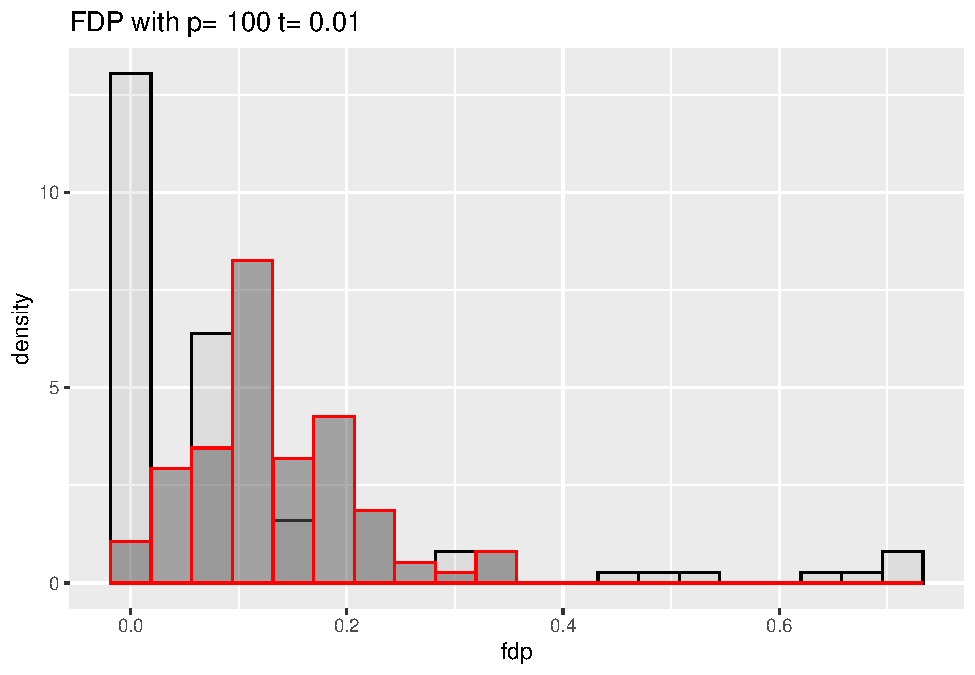
\includegraphics{Simulation_files/figure-latex/unnamed-chunk-1-1.pdf}

\begin{Shaded}
\begin{Highlighting}[]
\KeywordTok{my.fun}\NormalTok{(}\DataTypeTok{p=}\DecValTok{500}\NormalTok{, }\DataTypeTok{t=}\FloatTok{0.01}\NormalTok{)}
\end{Highlighting}
\end{Shaded}

\begin{verbatim}
## Warning in searchCommandline(parallel, cpus = cpus, type = type, socketHosts =
## socketHosts, : Unknown option on commandline: rmarkdown::render('/home/huihang/
## Documents/GWAS/Simulation.Rmd',~+~~+~encoding~+~
\end{verbatim}

\begin{verbatim}
## snowfall 1.84-6.1 initialized (using snow 0.4-3): parallel execution on 40 CPUs.
\end{verbatim}

\begin{verbatim}
## Library MASS loaded.
\end{verbatim}

\begin{verbatim}
## Library MASS loaded in cluster.
\end{verbatim}

\begin{verbatim}
## Library L1pack loaded.
\end{verbatim}

\begin{verbatim}
## Library L1pack loaded in cluster.
## 
## 
## Stopping cluster
\end{verbatim}

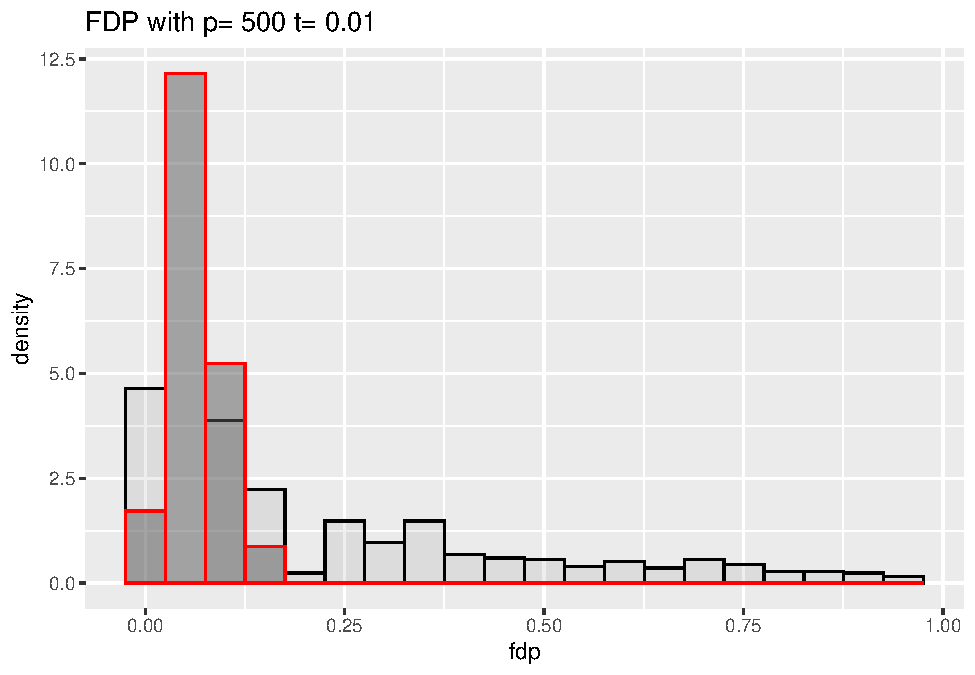
\includegraphics{Simulation_files/figure-latex/unnamed-chunk-1-2.pdf}

\begin{Shaded}
\begin{Highlighting}[]
\KeywordTok{my.fun}\NormalTok{(}\DataTypeTok{p=}\DecValTok{100}\NormalTok{, }\DataTypeTok{t=}\FloatTok{0.005}\NormalTok{)}
\end{Highlighting}
\end{Shaded}

\begin{verbatim}
## Warning in searchCommandline(parallel, cpus = cpus, type = type, socketHosts =
## socketHosts, : Unknown option on commandline: rmarkdown::render('/home/huihang/
## Documents/GWAS/Simulation.Rmd',~+~~+~encoding~+~
\end{verbatim}

\begin{verbatim}
## snowfall 1.84-6.1 initialized (using snow 0.4-3): parallel execution on 40 CPUs.
\end{verbatim}

\begin{verbatim}
## Library MASS loaded.
\end{verbatim}

\begin{verbatim}
## Library MASS loaded in cluster.
\end{verbatim}

\begin{verbatim}
## Library L1pack loaded.
\end{verbatim}

\begin{verbatim}
## Library L1pack loaded in cluster.
## 
## 
## Stopping cluster
\end{verbatim}

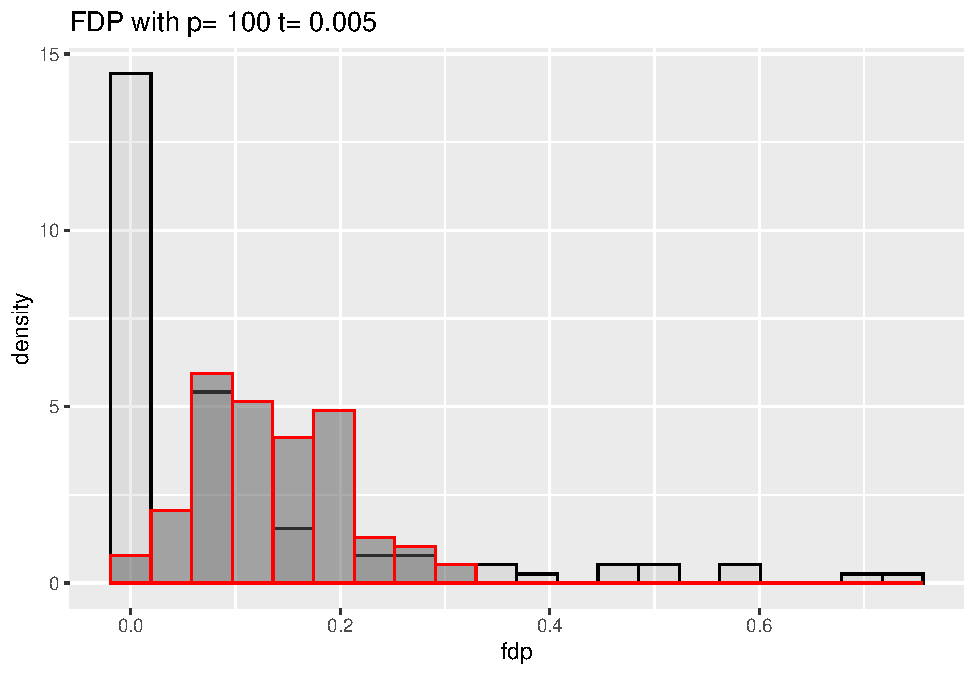
\includegraphics{Simulation_files/figure-latex/unnamed-chunk-1-3.pdf}

\begin{Shaded}
\begin{Highlighting}[]
\KeywordTok{my.fun}\NormalTok{(}\DataTypeTok{p=}\DecValTok{500}\NormalTok{, }\DataTypeTok{t=}\FloatTok{0.005}\NormalTok{)}
\end{Highlighting}
\end{Shaded}

\begin{verbatim}
## Warning in searchCommandline(parallel, cpus = cpus, type = type, socketHosts =
## socketHosts, : Unknown option on commandline: rmarkdown::render('/home/huihang/
## Documents/GWAS/Simulation.Rmd',~+~~+~encoding~+~
\end{verbatim}

\begin{verbatim}
## snowfall 1.84-6.1 initialized (using snow 0.4-3): parallel execution on 40 CPUs.
\end{verbatim}

\begin{verbatim}
## Library MASS loaded.
\end{verbatim}

\begin{verbatim}
## Library MASS loaded in cluster.
\end{verbatim}

\begin{verbatim}
## Library L1pack loaded.
\end{verbatim}

\begin{verbatim}
## Library L1pack loaded in cluster.
## 
## 
## Stopping cluster
\end{verbatim}

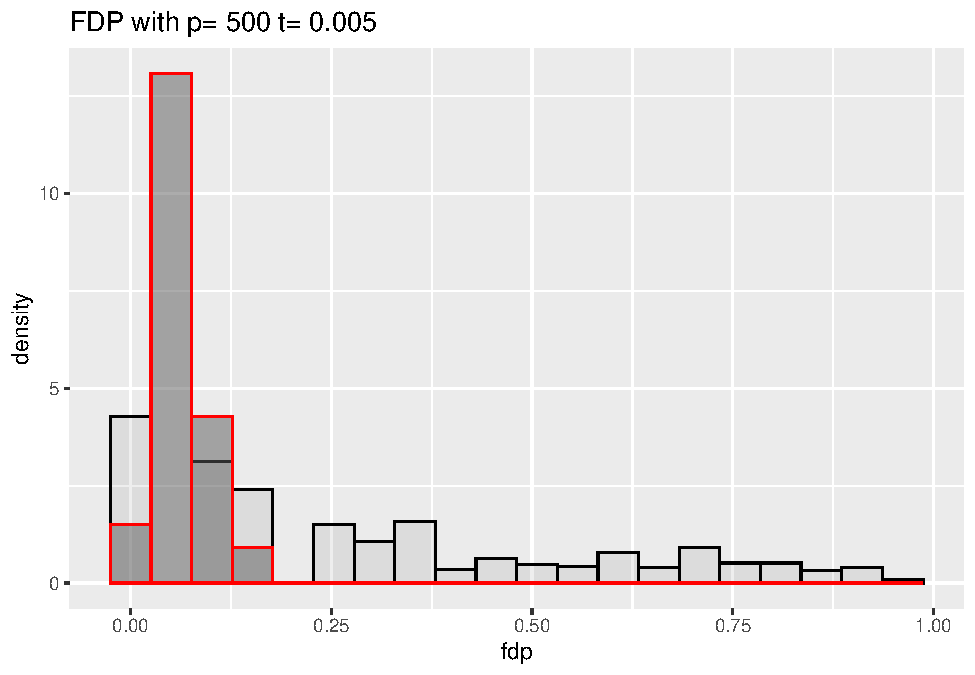
\includegraphics{Simulation_files/figure-latex/unnamed-chunk-1-4.pdf}

The grey bars in the figures is the density of \(FDR\) and the red bars
in the figures represent the density of \(\widehat{FDR}\).

From the figures above, I find both the true \(FDR\) and \(\widehat{FDR}\) are similiar with the result in the paper. 
I am satisfied with the result, althought they have some differences shown in the figure. 
But the paper just show the result of two factor model, so I cannot compare them.

I suppose it is because my \(\hat{W}\) is some kind of incorrect or biased, maybe. 


\end{document}
